\documentclass[12pt]{article}

\usepackage[margin=0.8 in]{geometry}
\usepackage{amsmath}
\usepackage{amssymb}
\usepackage{macros}
\usepackage{mathtools}
\usepackage{enumerate}
\usepackage{verbatim}
\usepackage{amsthm}
\usepackage{hyperref}

\title{}
%\content{}



\let \proj \undefined
\renewcommand{\tr}{ \mathrm{tr}}
\DeclareMathOperator{\SU}{SU}
\DeclareMathOperator{\proj}{proj}
\newcommand{\sS}{\mathscr{S}}
\DeclareMathOperator{\comp}{comp}
\newcommand{\A}{\mathcal{A}}
\renewcommand{\D}{\mathcal{D}}
\renewcommand{\e}{\epsilon}
\newcommand{\et}{\tilde{\e}}
\newcommand{\vr}{\mathbf{r}}
\newcommand{\vF}{\mathbf{F}}
\newcommand{\triple}{\iiint_E f(x,y,z)dV}



\newenvironment{solution}
  {\begin{proof}[Solution]}
  {\end{proof}
  
  }
\newtheorem{example}{Example}
\newtheorem{exercise}{Exercise}
\newtheorem{theorem}{Theorem}
\newtheorem{definition}{Definition}


\begin{document}
\section*{Cylindrical Coordinates}
What to know:
\begin{enumerate}
\item Be able to change from Cartesian to cylindrical and back.
\item Be able to set up and compute an integral in cylindrical coordinates.
\end{enumerate}


\subsection*{Motivation-Relations}
In a previous lecture we talked about polar coordinates, which was an alternative way of describing points on the $xy$ plane in a manner that made certain objects, such as annuli, sectors of disks and lines through the origin be easily described. For the next two lectures we'll describe two coordinate systems in the $xyz$ space that make particular objects easy to express.

To write a point of the $xyz$ space in Cylindrical coordinates, we first choose one of the axes (usually the $z$ axis)\footnote{The book defines cylindrical coordinates only with respect to the $z$ axis, but there isn't something particularly special about it; you can follow the same procedure with either the $x$ or $y$ axis.} as a reference, and all we have to do is keep the corresponding variable unchanged and change the other two into polar coordinates. 

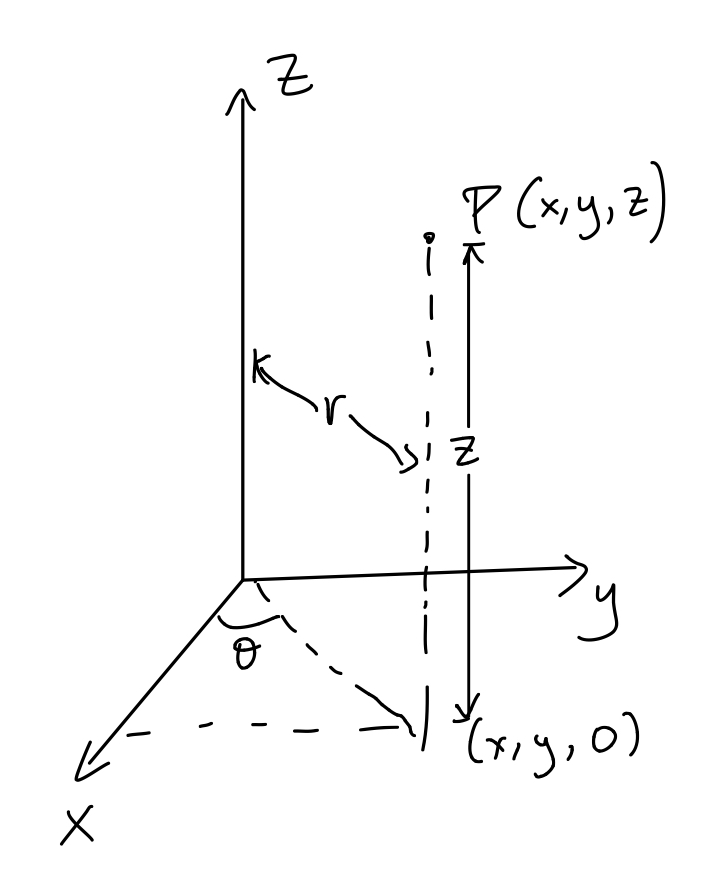
\includegraphics[scale=.2]{cylindrical.jpeg}
To be more specific about the process, say that we want to write a point in Cylindrical coordinates, written as $(r,\theta,z)$, with respect to the $z$ axis. Given a point $P(x,y,z)$, we project the point down to the $xy$ plane and find $(x,y,0)$. From previous lectures, we know that $(x,y)$ changes to polar coordinates using $x=r\cos(\theta) $ and $y=r\sin(\theta)$. So we find:
\begin{align*}
&x=r\cos(\theta) & r^2=x^2+y^2\\
&y=r\sin(\theta) & \tan(\theta)=\frac{y}{x}\\
&z=z & z=z
\end{align*}
\textbf{Remarks:} 
\begin{enumerate}
\item The notation for cylindrical coordinates might vary between authors, so it is a good idea to check with the author's definition if you're studying other books.
\item You can follow the link below to see a cute gif visualizing cylindrical coordinates. \url{https://en.wikipedia.org/wiki/File:Cylindrical_coordinate_surfaces.gif}
\end{enumerate}

\subsection*{Objects easily described in Cylindrical coordinates}
As we've seen already, polar coordinates allow us to write conveniently objects having some symmetry with respect to the origin. This leads to the expectation that cylindrical coordinates with respect to an axis will be useful for objects with some symmetry about this axis.

If we're talking about the $z$ axis, such objects are:
\begin{enumerate}
\item Cylinders of the form $x^2+y^2=r_0^2$, which can be turned into $r=r_0$.
\item Paraboloids of the form $z=x^2+y^2$, which become $z=r^2$.
\item Cones of the form $z^2=x^2+y^2$ which become $z^2=r^2$ (note that this allows $z$ being both positive and negative, as in an hourglass).
\item Spheres of the form $x^2+y^2+z^2=r_0^2$, that become $r^2+z^2=r_0^2$ (in the next lecture we'll see another coordinate system that is specifically tailored for spheres).
\end{enumerate}

\subsection*{Integration in Cylindrical coordinates}
The formula for an integral in Cylindrical coordinates with respect to the $z$ axis is quite predictable: nothing changes in $z$ and polar coordinates are used in $x, y$. We have:
\begin{theorem}
Let $E$ be a bounded domain in $\R^3$ written as $$E=\{(x,y,z): u_1(x,y)\leq z\leq u_2(x,y), (x,y)\in\D\}$$ where $$\D=\{(r,\theta):\alpha \leq \theta \leq \beta, h_1(\theta)\leq r\leq h_2(\theta)\},$$ and $f(x,y,z)$ continuous on $E$. Then $$\triple=\int_\alpha^\beta \int_{h_1(\theta)}^{h_2(\theta)}\int_{u_1(x,y)}^{u_2(x,y)} f(r\cos(\theta),r\sin(\theta),z)rdzdrd\theta.$$
\end{theorem}

\textbf{Remark:} Completely analogous theorems hold if you replace the $z$ axis with either $x$ or $y$ and do polar coordinates in the remaining two variables.

\begin{example} Find the volume of the solid $E$ bounded above by the paraboloid $z=2-x^2-y^2$ and below by the cone $z^2=x^2+y^2$, in the first octant.
\end{example}
\begin{solution}

Both surfaces are rotationally symmetric with respect to the $z$ axis, so we'll go for cylindrical coordinates with respect to the $z$ axis. We can write down our equations, solving for $z$:
\begin{align*}
&z=2-x^2-y^2\\
&z=\sqrt{x^2+y^2}\\
&z=0\\
&x=0\\
&y=0
\end{align*}

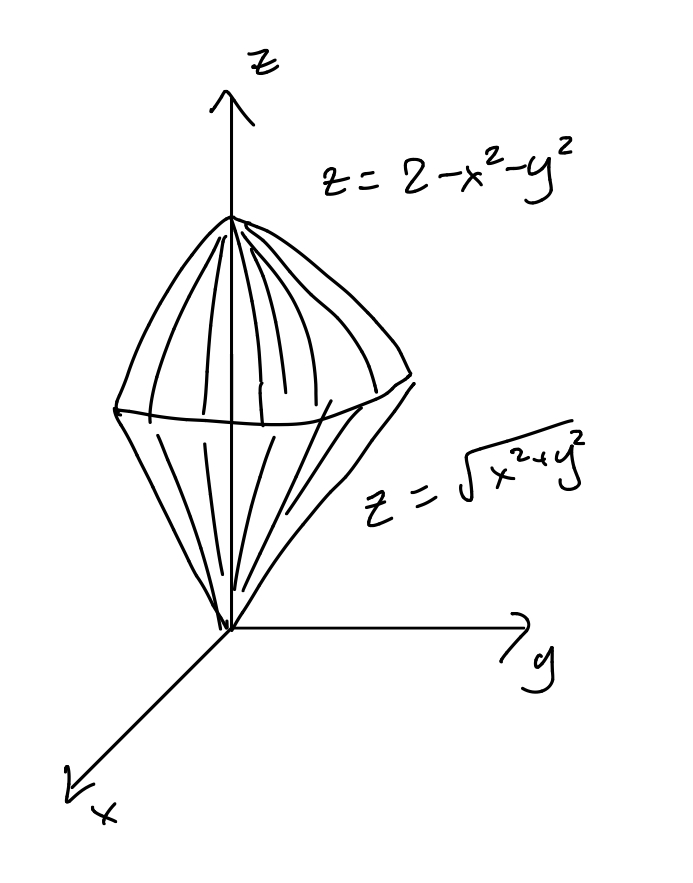
\includegraphics[scale=.2]{example.jpeg}
We can see from the picture that \begin{equation}\label{eq1}\sqrt{x^2+y^2}\leq z\leq 2-x^2-y^2,\end{equation} so $z=0$ is redundant. Then we need to look at the projection onto the $xy$ plane, so we intersect the first two equations and find $$\sqrt{x^2+y^2}=2-x^2-y^2.$$

To solve this equation, set $a=\sqrt{x^2+y^2}$ and treat it as a quadratic equation $a^2+a-2=0$, from which we find $a=1$ or $a=-2$, which can't be true because $a\geq 0$. So, we find that $x^2+y^2=1$ and, along with $x\geq 0$ and $y\geq 0$, we have that the projection is a quarter of the unit disk, so it can be written as $$\D=\{(r,\theta): 0\leq r\leq 1, 0\leq \theta\leq \pi/2\}.$$ 

In polar coordinates \ref{eq1} can be written as $$r\leq z\leq 2-r^2.$$ Finally: $$V(E)=\int_0^{\frac{\pi}{2}}\int_{0}^{1}\int_r^{2-r^2}rdzdrd\theta=\dots=\frac{5\pi}{24}$$


\end{solution}

\end{document}

